\documentclass{article}

\usepackage{amsmath}
\usepackage{amssymb}
\usepackage{tikz}
\usetikzlibrary{automata,positioning}

\title{Assignment 2}
\date{2019-01-24}
\author{MONTGOMERY, BENNET 20074049 CISC223\\
		\and GOEL, CHRISTOPHER 20053408 CISC223\\
		\and VIOLO, JARED 20051382 CISC223\\
		\and DALLAS, SPENCER 20048480 CISC223}


\begin{document}
	\maketitle
	\pagenumbering{arabic}
	
	\section*{Q1.}
	\subsection*{(a)}
	Three strings that are accepted by the state diagram are 00, 0110, and 0101. Three strings that are not accepted by the state diagram are 01, 010, 0100.
	\subsection*{(b)}
	\begin{table}[ht]
		\caption{Transition Table}
		\centering
		\begin{tabular}{ c | c c }
			\hline
			\hline	
			Current State & input 0 & input 1 \\
			\hline
			A & B & C \\
			B & A & D \\
			C & D & A \\
			D & C & B \\
			\hline
		\end{tabular}
	\end{table}
	\subsection*{(c)}
	The language of the diagram consists of the set of all strings with an even number of 1s and an even number of 0s.
	
	\section*{Q2.}
	Node $E$ is linked to node $F$ in $M$ by $\epsilon$, and $F$ is linked to $E$ by the real transition $b$, therefore we can write a transition from $E$ to $E$ with $b$ in $M'$. Since node $F$ is linked to node $G$ in $M$ by $\epsilon$, and $G$ is linked to $F$ by the real transition $a$, therefore we can write a transition from $F$ to $F$ with $a$ in $M'$. Node $E$ is linked to node $F$ by $\epsilon$, node $F$ is linked to node $G$ by $\epsilon$, and node $G$ is linked to node $F$ through real value $a$ in $M$, that is to say there is an $\epsilon$ chain of length 2 ending in real value $a$. This allows us to connect $E$ to $F$ directly in $M'$. Finally, since there is a chain of length 1 $\epsilon$-transitions between node $E$ and node $F$ in $M$ and node $F$ is an accepting state, $E$ becomes an accepting state in $M'$. Putting this all together gives us the following final diagram:\\
	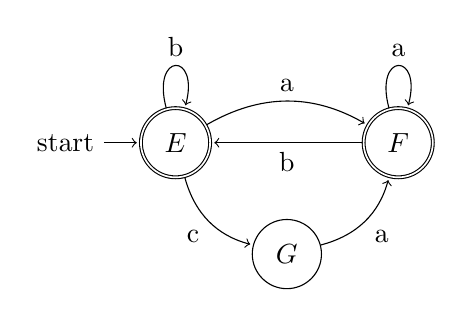
\begin{tikzpicture}[shorten >=1pt,node distance=2cm,on grid,auto] 
   		\node[state,initial,accepting] (E)   {$E$};  
   		\node[state] (G) [below right=of E] {$G$};
   		\node[state,accepting] (F) [above right=of G] {$F$};
    	\path[->]
    	(E) edge [bend right] node [swap] {c} (G)
    		edge [bend left] node {a} (F)
          	edge [loop above] node {b} ()
    	(G) edge  [bend right] node [swap] {a} (F)
    	(F) edge  node {b} (E) 
          	edge [loop above] node {a} ();
	\end{tikzpicture}
	
	\section*{Q3.}
	The following state/input subset table is derived from the NFA in question 3:
	\begin{table}[ht]
		\centering
		\begin{tabular}{ c | c c }
			State & Input a & Input b \\
			\hline
			\{1\} & \{2\} & \{3\}\\
			\{2\} & \{3\} & \{4\}\\
			\{3\} & \{1,2\} & \{3\}\\
			\{4\} & \{2\} & \{3,4\}\\
			\{1,2\} & \{2,3\} & \{3,4\}\\
			\{2,3\} & \{1,2,3\} & \{3,4\}\\
			\{3,4\} & \{1,2\} & \{3,4\}\\
			\{1,2,3\} & \{1,2,3\} & \{3,4\}\\
		\end{tabular}
	\end{table}
	
	The DFA resulting from this table is:\\
	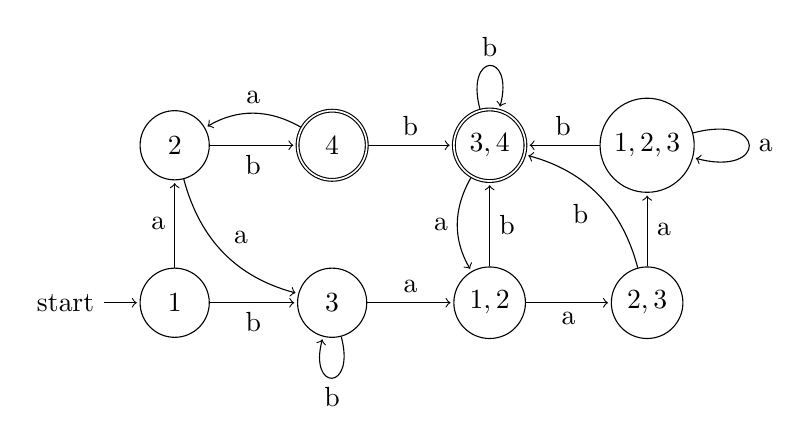
\begin{tikzpicture}[shorten >=1pt,node distance=2cm,on grid,auto] 
		\node[state,initial] (1) {$1$};
		\node[state] (2) [above=of 1] {$2$};
		\node[state] (3) [right=of 1] {$3$};
		\node[state,accepting] (4) [right=of 2] {$4$};
		\node[state,accepting] (34) [right=of 4] {$3, 4$};
		\node[state] (12) [right=of 3] {$1, 2$};
		\node[state] (23) [right=of 12] {$2, 3$};
		\node[state] (123) [right=of 34] {$1, 2, 3$};	
		\path[->]
		(1) edge node {a} (2)
			edge node [swap] {b} (3)
		(2) edge node [swap] {b} (4)
			edge [bend right] node {a} (3)
		(3) edge node {a} (12)
			edge [loop below] node {b} (3)
		(4) edge [bend right] node [swap] {a} (2)
			edge node {b} (34)
		(12) edge node [swap] {b} (34)
			 edge [swap] node {a} (23)
		(23) edge node [swap] {a} (123)
			 edge [bend right] node {b} (34)
		(34) edge [bend right] node [swap] {a} (12)
			 edge [loop above] node {b} ()
		(123) edge node [swap] {b} (34)
			  edge [loop right] node {a} ();
	\end{tikzpicture}
\end{document}